\section{\todo{Discussion}}\label{6_discussion}
\begin{comment}
The present study aimed at investigating whether an interactive slackline training system, which 


- results discussion (sport activity people)

- results discussion (lateral preference)

- results discussion (gender)

- observation on study during training

- interview
\end{comment}

\subsubsection{Interaction effects}
No interaction effect for group x time can be shown for any measurement variable for the ISG or the HTG.
This means that no group is better or worse than the other in any measurements.
Therefore the hypothesis that the interactive system shows better results than a human trainer cannot be proven with a statistically significant.
Looking at the figures of the improvements for the group in each measurement \ref{fig:6_4_standImprovement}, \ref{fig:6_4_stepsImprovement}, and \ref{fig:6_4_distanceImprovement}, no real difference can be seen between the groups.
The ISG group is at the most time slightly better in all conditions, which is not sufficient to prove a statistically significance.
A bigger difference can be shown in terms of the right leg side for the walked steps (figure \ref{fig:6_4_stepsRightImprovement}) and walked distance measurements (figure \ref{fig:6_4_distanceRightImprovement}).
It shows that the ISG is approximately 2.5 times better for the right leg.
However the standard deviation of each group is very large, so that it is also not sufficient to have a certain significance.

Since all significance values are larger the defined alpha value of 0.05, the null hypothesis cannot be rejected.
This means that no interaction effect can be found over time from pre to post measurements comparing the groups ISG and HTG and therefore no group is better or worse than the other one.
This can be caused by multiple reasons.
%- Übung zu kurz um unterschied festzustellen

The duration of the training could have been too short to show a statistically significant difference between the groups.
All participants learned just basic techniques of slacklining but no further slackline skill has been trained.
For learning more complex exercises and techniques especially the introduction and feedback given during the execution is very important, since these are key elements of understanding how the exercise works and how to perform it correctly.
Therefore further exercises and further training over a longer time range  could lead to a more specific result, 
%The only difference lied in the effect of how to provide the subject with important information and how to give her feedback about the actual performance.

%- test in zu kurzer zeitspanne um unterschied festzustellen
Second, the participants could have been too exhausted for showing a relevant effect.
Participants trained at least 45 minutes on the slackline.
After this the post measurement has been executed.
Since the training lasted minimum one hour, the measurement results after the training could have been affected by the exhaustion of the participants and therefore not showing there real improvement.
%because of the training could weaken the participant and therefore show not the expected results of an improvement.
%There could be a side effect that participants won't be able to show there real improvements directly after the training due to exhaustion.

%- Unterscheidung zwischen grundlegender balancefähigkeit nicht gemacht somit randomisierte ergebnisse
%alle participants anfgäner auf slackline und keine weiteren ablancetraining bla
% aber nicht nach grundlegenden balanceskill geschaut
% ist bei jedem anders, einer is besser der andere schlechter 
% im test aufgefallen, dass es gute, mittelmäßige und schlechte participants gibt, was sich in der standardabweichung wiederspiegelt
% wennn man die in gruppen einteilen würde bzw auf darauf prüfen würde wie gut die grundlegende balancefähigkeit ist, hätte man ein eingeschränkteres ergebnis, welches die std dev verringert und somit auf signifikanz kommen könnte


Lastly, there was no distinction in general balance skill of the participants.
Subjects were chosen if they had no intermediate slackline experience (i.d. tried slacklining at most two times) or no further balance skill through special sport activities.
The results show a large standard deviation for all variables in the difference of pre to post, because participants improved differently after the training respectively to their pre measurement.
This means that subjects show different general balance characteristics.
Therefore for further studies it is recommended to test on the general balancing skill and characteristic of the participants, to minimize the chance of randomized data because of not qualified participants.

% --> differ the characteristic of balance improvement to reduce randomized data
% --> no distinction in general balance skill
%Third, all participant had to make single leg stance on a common floor and on a rolled towel, which served for validating that no participants has a balance disorder.
%Another reason could be that no grouping of general balance skill has been done.
%In the study only a general distinction of no prior slackline, further balance experience, or balance disorder has been done.

%- dennoch sehr leichter trend für ISG zu verbesserung
However a trend can be observed, that the ISG improved slightly better in numerical average than the HTG.
This could be the case, because the system's gesture recognition is less tolerant about the exercise execution than a human trainer
Whereas a trainer is more tolerant about the users exercise execution, the system has a predefined gesture database, to which the user has to adapt herself.
It leads to more trial executions, because of the strict recognition of the system.

\subsubsection{Time effects}
The time effect seen in table \ref{tab:6_4_mainEffects} in the column \textit{Time} shows whether it differs significantly from pre to post measurement, without considering any group.
This means the time effect is observed for all participants as one entity, like no group would exist.
The results state for all measurement conditions a significant improvement, unless for stand left.
With this it is proven that the used training exercises by both groups are useful and have an effect on the improvement of the participant.

The standing left leg showed no statistically significant result ($p$ = 0.078).
It is more difficult to hold the balance on a weaker leg, because it is less familiar with handling these situations than the primary leg.
Since slacklining is a more complex balance activity, the general balance of the trainee has to be trained with her weaker leg to show an improvement of the slackline specific training.
It can be assumed that less trained legs or participants won't show an improvement as good as participants or legs that have a certain general sense of balance.
Furthermore the physical strain could have exhausted the functionality of the leg, since post results has been measured directly after the training.

In reverse the right leg shows significant results.
For all participants their right leg was the primary leg.
The general balance skill for this leg is given through everyday physical effort and therefore it shows more stable data for balance improvements.

\begin{figure}[htb]
	\centering
	\begin{minipage}[t]{0.32\linewidth}
		\centering
		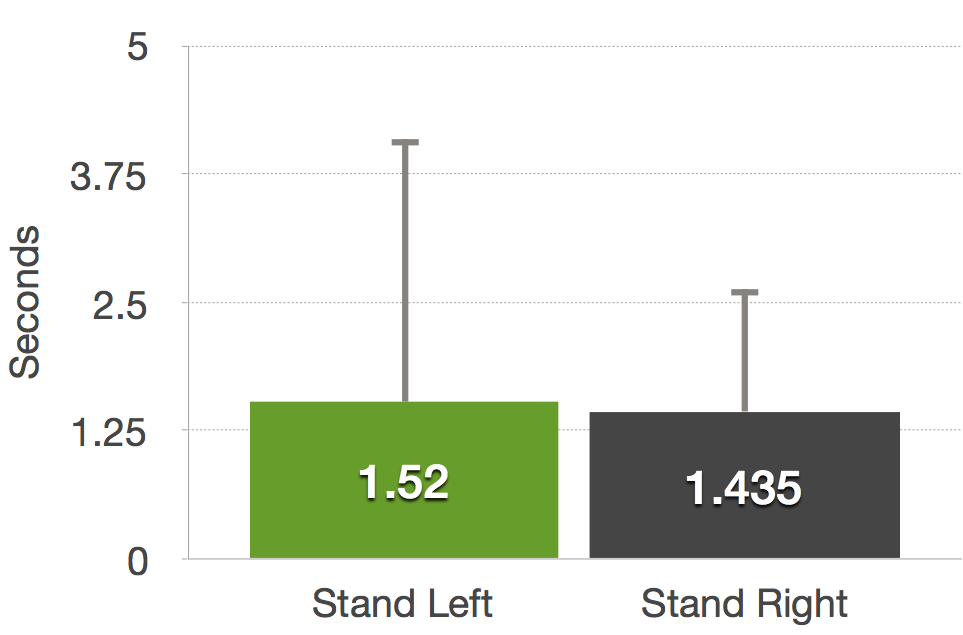
\includegraphics[width=1\linewidth]{Pictures/6_4_DIA_StandAllDiff}
		\subcaption{Improvement on Distance with Left Starting Leg}
		\label{fig:6_4_standAllDiff}
	\end{minipage}
	\hfill
	\begin{minipage}[t]{0.32\linewidth}
		\centering
		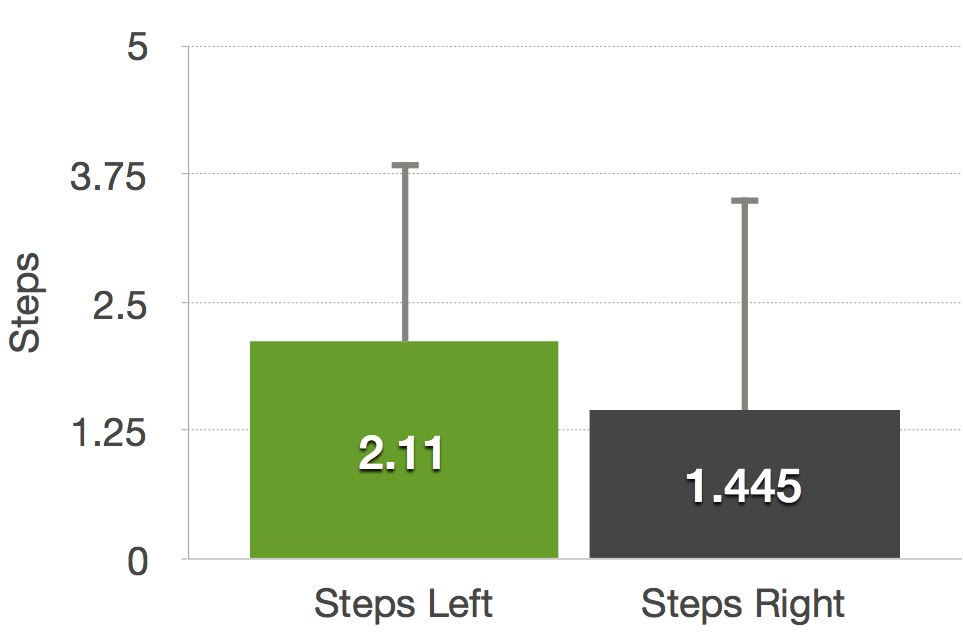
\includegraphics[width=1\linewidth]{Pictures/6_4_DIA_StepsAllDiff}
		\subcaption{Improvement on Distance with Right Starting Leg}
		\label{fig:6_4_stepsAllDiff}
	\end{minipage}
		\hfill
	\begin{minipage}[t]{0.32\linewidth}
		\centering
		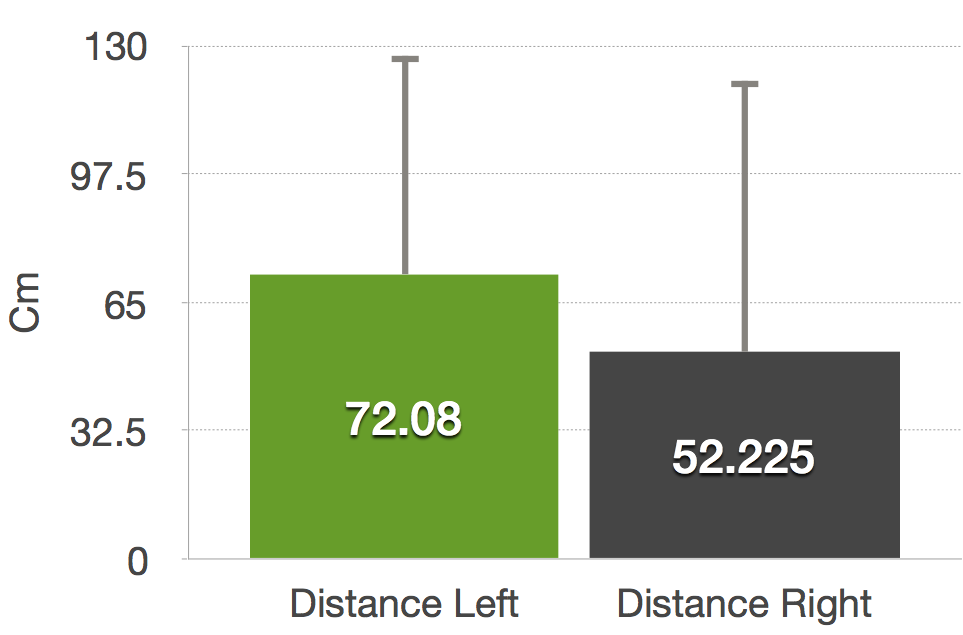
\includegraphics[width=1\linewidth]{Pictures/6_4_DIA_DistanceAllDiff}
		\subcaption{Improvement on Distance with Right Starting Leg}
		\label{fig:6_4_distanceAllDiff}
	\end{minipage}
	\caption{Walked Distance Improvement}
	\label{fig:6_4_distanceImprovement}
\end{figure}

\subsubsection{Group effect}
The main effect for the group is analogue to the previous main effect of the time.
With this, the differences between groups can be calculated, without considering the time.
Looking at table \ref{tab:6_4_mainEffects} in column \textit{Group}, no significant effect can be seen.
This means no group differs from each other.
The diagrams in figure \ref{fig:6_4_mainEffectGroup} show that all results are relatively similar.
Although the ISG is numerically slightly better than the HTG it is not sufficient to have a statistically significance difference.
%no difference calculated
% pre nicht in betracht gezogen
%keine verbesserung der teilnehmer betrachtet
\begin{figure}[htb]
	\centering
	\begin{minipage}[t]{0.40\linewidth}
		\centering
		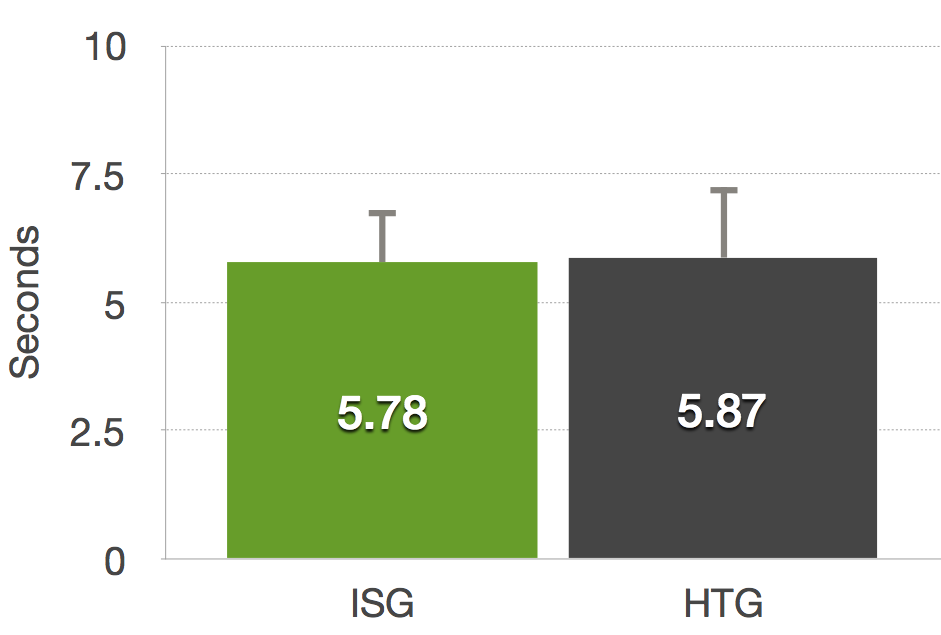
\includegraphics[width=1\linewidth]{Pictures/6_4_DIA_StandLeftGroupEffect}
		\subcaption{Stand Left Results}
		\label{fig:6_4_standLeftGroupEffect}
	\end{minipage}
	\hfill
	\begin{minipage}[t]{0.40\linewidth}
		\centering
		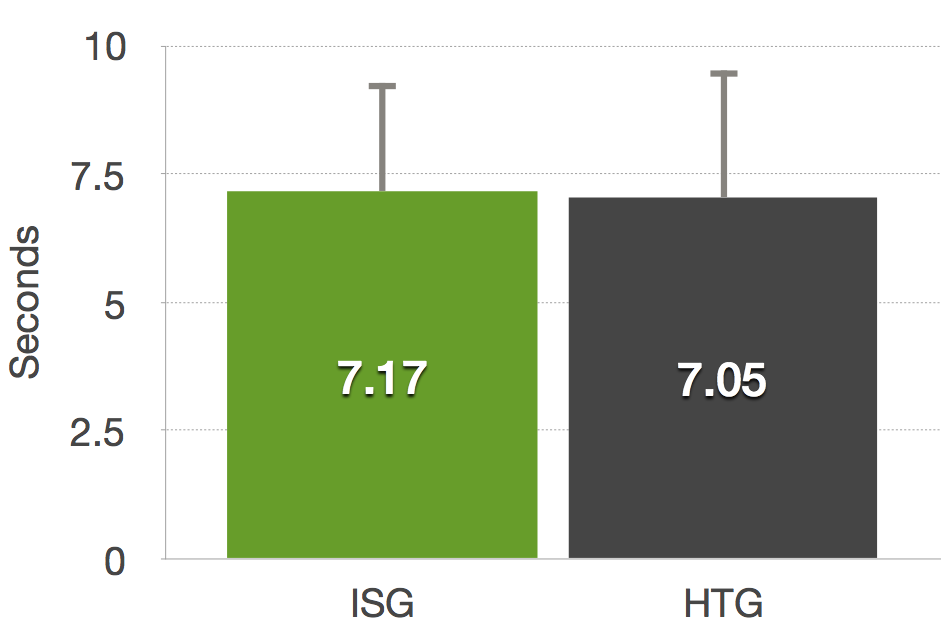
\includegraphics[width=1\linewidth]{Pictures/6_4_DIA_StandRightGroupEffect}
		\subcaption{Stand Right Results}
		\label{fig:6_4_standRightGroupEffect}
	\end{minipage}
	\hfill
	\begin{minipage}[t]{0.40\linewidth}
		\centering
		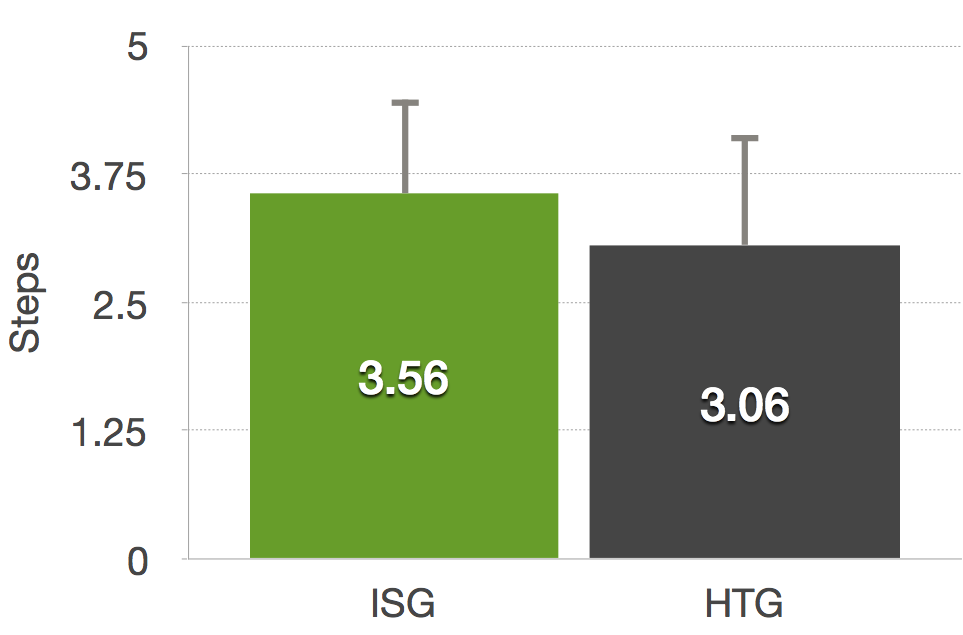
\includegraphics[width=1\linewidth]{Pictures/6_4_DIA_StepsLeftGroupEffect}
		\subcaption{Steps Left Results}
		\label{fig:6_4_stepsLeftGroupEffect}
	\end{minipage}
	\hfill
	\begin{minipage}[t]{0.40\linewidth}
		\centering
		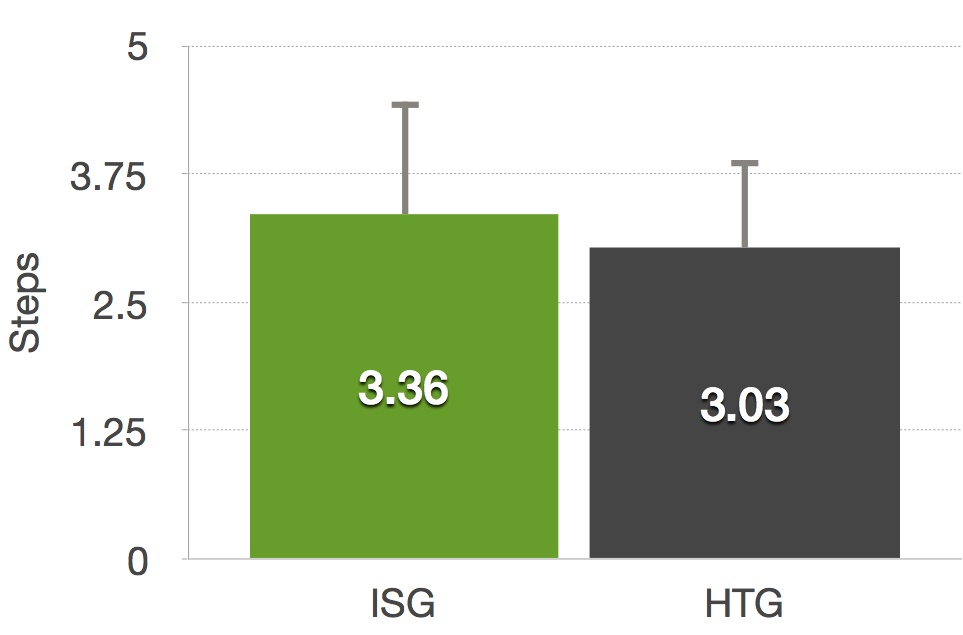
\includegraphics[width=1\linewidth]{Pictures/6_4_DIA_StepsRightGroupEffect}
		\subcaption{Steps Right Results}
		\label{fig:6_4_stepsRightGroupEffect}
	\end{minipage}
	\hfill
	\begin{minipage}[t]{0.40\linewidth}
		\centering
		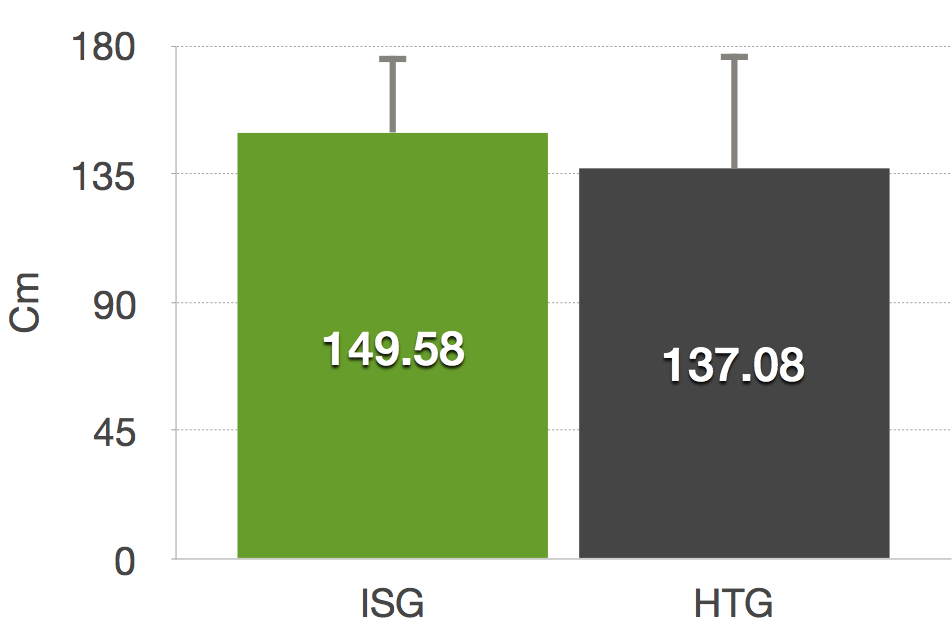
\includegraphics[width=1\linewidth]{Pictures/6_4_DIA_DistanceLeftGroupEffect}
		\subcaption{Distance Left Results}
		\label{fig:6_4_distanceLeftGroupEffect}
	\end{minipage}
	\hfill
	\begin{minipage}[t]{0.40\linewidth}
		\centering
		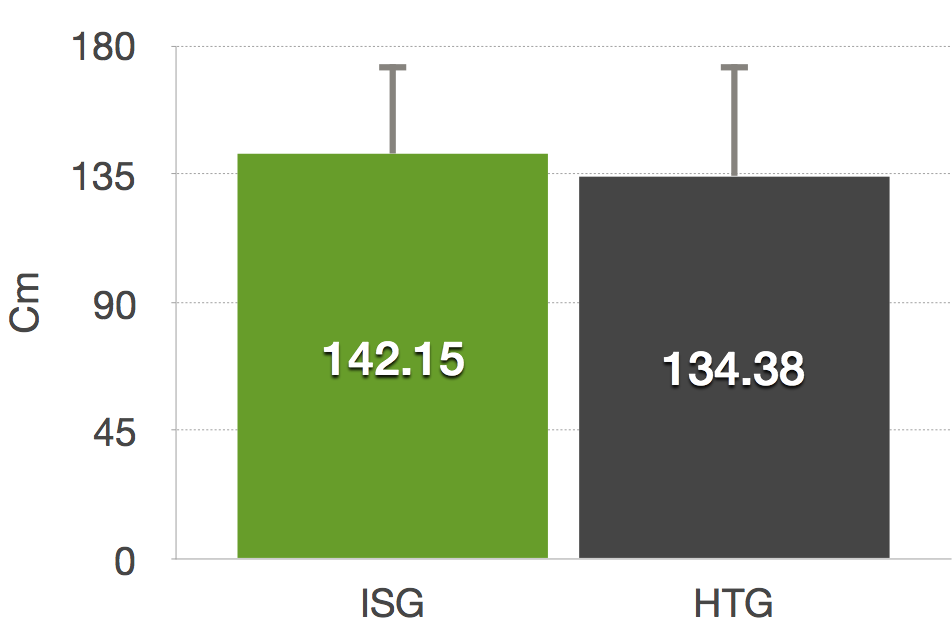
\includegraphics[width=1\linewidth]{Pictures/6_4_DIA_DistanceRightGroupEffect}
		\subcaption{Distance Right Results}
		\label{fig:6_4_distanceRightGroupEffect}
	\end{minipage}
	\caption{Scores for comparing the main effects of the group}
	\label{fig:6_4_mainEffectGroup}
\end{figure}

\subsubsection{Slackline Training Observations}\label{6_4_slacklineObservations}
During the training some observations have been made that would be useful to consider for further practice with the interactive slackline system.

A participant showed up with black pants, which resulted into problems with the Kinect tracking recognition.
This is because some black clothing absorb the infrared light of the Kinect, which makes the trackability more difficult \cite{KinectBlackClothing}.
It would be helpful to indicate participants to not wear any black clothes.

Concerning the exercises there were problems with tracking the participants while sitting on the slackline (Figure \todo{Figure exercise}).
Five out of six participants had problems with this exercise.
Almost all participants out of both groups noted that the sitting exercises are very uncomfortable.
Because of the way the problem exist, this exercise should be eliminated from the exercise list or replaced with exercises to train going up on the slackline.
Like seen in figure \todo{Figure exercise} the leg of the participant was mistaken with the slackline by the Kinect.

The very last exercise resulted also in tracking problems with four out of six participants (Figure \todo{figure}).
Here they had to walk two steps forward on the slackline.
A general problem was the up going on the slackline.
If the leg was too close to the line while going up, the Kinect did not tracked it appropriately.
Both problems could be fixed by tracking the gestures with more persons that execute different variations of a correct exercise execution.

Three participants in the ISG had especially problems with scrolling the exercise list at the beginning because they didn't know how to interact with it.
Adding an introduction on how to scroll a list in the system could be helpful.

\subsubsection{Subjects Rating of exercise difficulty}
Participants were asked to rate exercises after finishing a set of exercises with both legs.
They could choose a difficulty on a scale from 1 (very easy) to 5 (very difficult).
The ratings of all participants were averaged.
Figure \ref{fig:6_4_exerciseDifficulty} shows the ratings of each exercise (blue line) as well as a trendline, which is a linear interpolation of the values (green line).

\begin{figure}[htb]
	\centering
	\begin{minipage}[t]{0.92\linewidth}
		\centering
		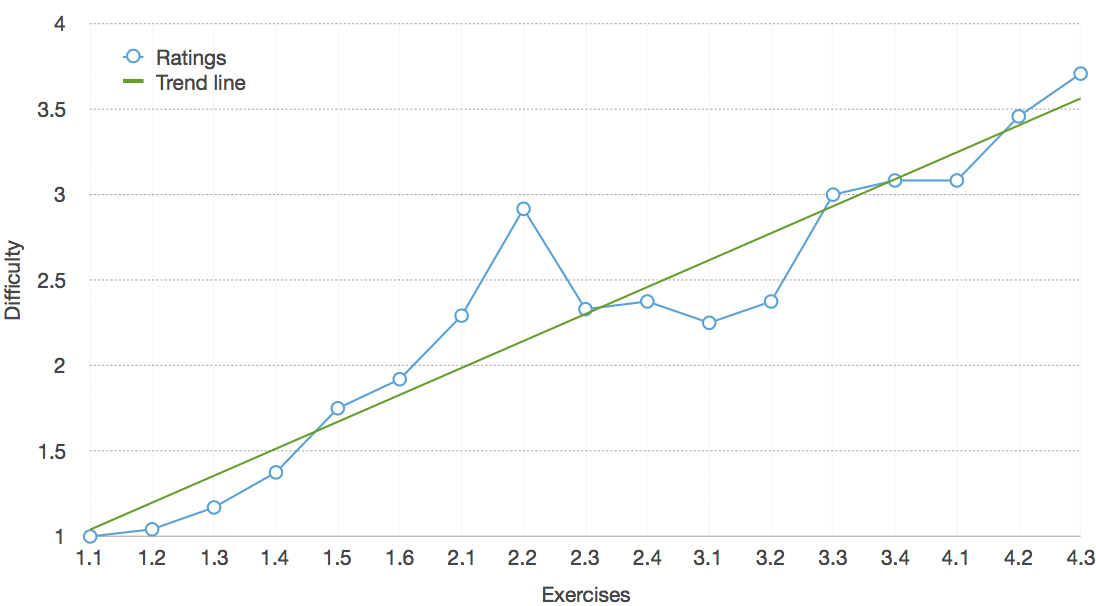
\includegraphics[width=1\linewidth]{Pictures/6_4_DIA_ExerciseDifficulty1}
		\caption{Study groups example}
		\label{fig:6_4_exerciseDifficulty}
	\end{minipage}
\end{figure}

The exercises of the first level follow a smooth increase in difficulty, which matches also the idea of strengthen the general balance skill of the participants and preparing them for standing on a slackline.
For the second level there is a massive increase in difficulty for the first two exercises.
This corresponds also with the observations in section \textit{\nameref{6_4_slacklineObservations}}, where participants claimed that the exercise is very uncomfortable or too difficult for them.
Exercises 2.3, 2.4, 3.1, and 3.2 show similar ratings.
This is because they are all very similar exercises, in which the participant learned to go up on the line.
However the time was increased for exercise 3.1 and 3.2.
Some participants noted that they felt more secure to stand longer on the slackline after doing the short-time exercises.

The ratings follow a linear ongoing trend and therefore verify the appropriate integration of exercises as an entire training model for beginners on a slackline.


\subsubsection{Semi-structured Interview}
The general experience with the training method showed similar outcomes for both groups. 
They felt a positive learning progress during the training and had a sense of achievement through challenging but practicable exercises.
%Representative participant 10 said: \textit{"The Exercises were well-framed. I felt a learning progress. At the beginning i was not aware of the whole body balance but after the training it could feel how the body balance changed and how I could keep my body in the center of gravity."}

Participant 3 (ISG) mentioned further \textit{"[...] There is no need to watch YouTube tutorials with such a system. It displays all relevant information and provides appropriate feedback"}.
Participant 4 and 6 (ISG) said a personal trainer could be more helpful for giving more specific advises that the Kinect could not detect.
%answered \textit{"Yes because I have learned something and I do not have to watch YouTube tutorials because it tells me whether I am wrong or not. The user view is also helpful during the exercise execution"}. Participant 4 (ISG) mentioned \textit{"For beginners very well because you can feel and see your own progress through unlocking the exercises. Although a personal trainer could mention things that the Kinect won't detect"}.

The most annoying experience for the ISG was the partially bad gesture recognition of the Kinect and the interaction with it, whereas in the HTG participant 10 mentioned missing exercises for how to get up on the slackline and participant 12 noted especially the uncomfortableness of the sitting on the slackline exercises.

On the other hand they liked the environment design, clear description and especially the looping videos of the exercises as well as the appropriate feedback during the execution.
Participant 6 mentioend further \textit{"I liked the user view because you can see how you act by yourself. Also I can use the system without any further help"}

Lastly a various amount of application scenarios for the interactive training system were mentioned.
Most mentioned physiotherapy, rehabilitation, in general as training for sport activities, gym, and home trainer.